\documentclass[../thesis.tex]{subfiles}
\begin{document}
\chapter{Integrated Photoluminescence Lifetimes} \label{sec:integrated_lifetime}
As OLEDs become fully a fully commercialized technology, several challenges still exist that need to be overcome to realize full potential.
Chief among these is the operational lifetime, which has been a key focus of recent studies.\supercite{Scholz2015,DeMoraes2011,Seifert2013b,Moraes2011,Burrows1994,Seifert2013b}
Lifetime is typically characterized at constant current density, recording the luminance loss and voltage as a function of time.
The lifetime is then reported as the time to reach some arbitrary fraction of the initial luminance.
Unlike the steady-state efficiency, it is difficult to optimize a device lifetime by brute force.  
Due to the long lifetime of devices, even under accelerated aging, it takes a substantial amount of time to characterize devices and iteratively improve a design.
This reality makes it essential to have a deeper insight into the processes that are limiting lifetime.

While this simple lifetime characterization is effective for device to device comparison, further insight into the mechanism is found wanting.
Modeling techniques are used extensively for degradation characterization, using the mechanisms outlined in Chapter \ref{sec:degradation_mechanisms}.\supercite{Giebink2008a,Ingram2017,Coburn2017}
While these techniques are able to reproduce the decay characteristics with a root in physical mechanisms, they suffer from over-parameterization and introduce parameters that cannot be experimentally confirmed.
As discussed in Chapter \ref{sec:degradation_analysis}, a variety of chemical, structural, and spectroscopic techniques are often employed to gain further insight into the physical processes.\supercite{Seifert2013b,Moraes2011,Scholz2015,Wang2011a,Zhang2016}
These techniques can be insightful, but are difficult to apply on a large scale due to the additional processing time.
Post degradation analysis does not provide a temporal characterization of degradation without processing individual devices at several decay points, which can be extremely time consuming.
Additionally, it may be helpful to categorize luminance loss into different luminance loss pathways, which few of these techniques are able to do.
It would be beneficial to have a technique that is able to provide more information during the degradation, without increasing experimental time, as well as provide a way to decouple loss pathways.
This is done by introducing an optical pump to independently measure \pl as a function of time.
Similar techniques have been utilized before, but have lacked completeness in their care to treat assumptions, as well as their resolution.\supercite{Popovic2001,Kondakov2007d,Winter2008a}


This chapter demonstrates a method for decoupling the device photoluminescence loss from the exciton formation losses during operational lifetime testing.  
This is a summary and extension of my work entitled \textit{Decoupling degradation in exciton formation and recombination during lifetime testing of organic light-emitting devices}.\supercite{Hershey2017}


\section{Luminance as Efficiency Loss}

When OLEDs are degraded at constant current density, luminance loss is observed.  
As discussed in Chapter \ref{sec:efficiency_analysis}, quantum efficiency is the ratio of photons leaving the device per electron input.
Therefore, at constant current density (or constant electron flux), luminance loss is actually an efficiency loss.
Chapter \ref{sec:unified} extensively discussed a revised formalism for understanding OLED efficiency.
In particular, we will take advantage of the formalism of exciton formation efficiency.  
For decoupling luminance loss pathways, a categorical expression for \eqe is desired, rather than the dynamics approach taken in Equation \ref{eqn:eqeReform}, therefore Equation \ref{eqn:eqeSimple} is modified to include a quenching term, yielding

\begin{equation}
\eqe=\pl\oc\chi\ef\eta_\tau
\label{eqn:eqe_quenching}
\end{equation}

where $\eta_\tau$ is the fraction of excitons that relax via the natural exciton lifetime, $\tau$.  
this term is current-density dependent and captures the quenching events discussed in Chapter \ref{sec:unified}.
It is also important to note that during degradation, \ef captures not only the previously discussed polaron loss due to leakage events, but also the formation of non-radiative recombination centers (NRRCs).
NRRCs are states that form excitons off of the emissive molecule and allow charge recombination without forming light, which have been shown to be present in degrading devices.\supercite{Kondakov2003,Kondakov2007d}
The interpretation of \ef as the exciton formation efficiency needs to be clarified to be the efficiency of exciton formation on the emissive molecule, but remains otherwise unchanged.

During degradation, to categorize efficiency loss, each term in Equation \ref{eqn:eqe_quenching} could be considered to be time dependent.  
However, it is reasonable to assume that some of these terms are unchanged, or have minimal impact.
The exciton's radiative spin fraction, $\chi$ is a quantum mechanical property of the emissive molecule.
Therefore, without changes in the emissive molecule, this term should remain constant.  
If emission from another state was observed spectrally, this would indicate a need to adapt Equation \ref{eqn:eqe_quenching} for multiple emissive states, greatly complicating this process.
Thankfully, that is of yet unobserved in our research.


\begin{wrapfigure}{r}{.5\textwidth}
    \begin{minipage}{\linewidth}
    \centering%\captionsetup[subfigure]{justification=centering}
    \includegraphics[width=0.48\textwidth]{integratedLifetime/microscope}
    %\subcaption{}
    %\label{fig:5a}\par\vfill

    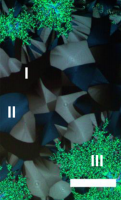
\includegraphics[width=0.48\textwidth]{integratedLifetime/crystals}
    %\subcaption{}
    %\label{fig:5b}
\end{minipage}
\caption{Cross polarized optical micrographs of (a) active device area (b) crystallized film from Fielitz \textit{et al.}.\supercite{Fielitz2016}
(I) Orthorhombic phase, (II) Triclinic Phase, (III) 200 $\mu$m scale bar}
\label{fig:micrographs}
\end{wrapfigure}

The out-coupling efficiency, \oc, is a property dependent on the layer optical constants and thicknesses.
Without significant changes in molecular composition and morphology, it is unlikely that \oc should change.
The most likely was to create these changes would be through crystallization.  
This can be investigated by looking at the devices under crossed polarized optical microscopy.\supercite{Fielitz2016}
Figure \ref{fig:micrographs} shows that in our devices, no crystallization is observed.
The reference photo, taken from Fielitz \textit{et al.}\supercite{Fielitz2016} demonstrates how apparent crystallization would be if present.
It is also important to note that \oc depends on the emitter distribution within the device, and thus the recombination zone.
If there is a shift in RZ, out-coupling is likely to change.  
It is difficult to assess recombination zone and unprecedented to measure as a function of degradation.
However, this problem is minimized in thin emissive layers, so studies should attempt to focus on thinner EML devices to reduce error.

Lastly, $\eta_\tau$ is assumed to be constant for this work since it cannot be measured quantitatively.
An approximation of the impacts of this term are discussed in Section \ref{sec:eta_tau}

With these terms assumed to be constant, the only time dependent terms are \pl and \ef, and the time dependent version of Equation \ref{eqn:eqe_quenching} can be written as


\begin{equation}
\frac{\eqe(t)}{\eqe^0}=\frac{\pl(t)}{\pl^0}\frac{\ef(t)}{\ef^0}
\label{eqn_eqe_decay_components}
\end{equation}

where $X^0$ is the initial value of the parameter before degradation.
Since $\eqe(t)$ is the luminance loss as a function of time, an independent measurement of \pl would allow a full decoupling of \eqe into \pl and \ef.

\section{Photoluminescence Characterization}
\begin{figure}[ht]
\centering
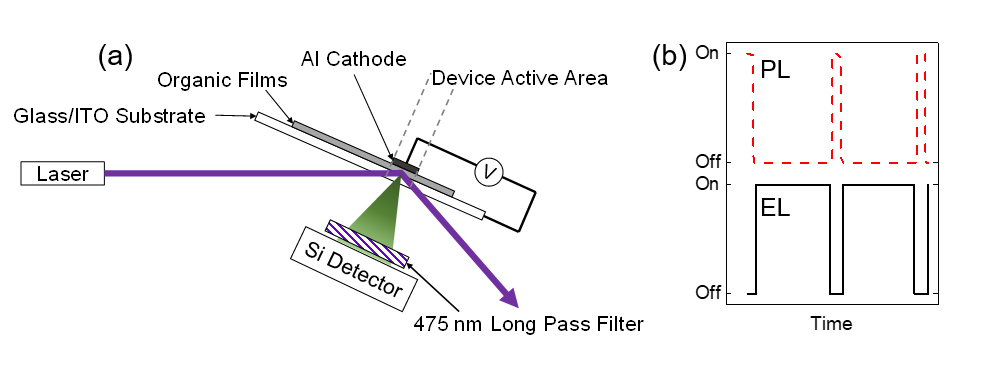
\includegraphics[width=0.8\textwidth]{integratedLifetime/schematic}
\caption{(a) Experimental configuration for the measurement of electro- (EL) and photoluminescence (PL) during OLED degradation.  Laser excitation is incident on a subsection of the device area.  The laser is aligned so that neither the incident nor reflected beam strikes the detector.  Stray laser light is removed by a $\lambda$=475 nm dielectric long pass filter.  (b) Excitation scheme.  EL and PL signals are probed independently with no temporal overlap.  (c) External quantum efficiency versus current density and luminance for devices having emissive layer thickness of 10 nm, 20 nm and 30 nm.}
\label{fig:schematic}
\end{figure}

In order to independently measure \pl during degradation, intermittent optical excitation is done using a laser, as shown in Figure {fig:schematic}a.
The laser forms as 1mm diameter circular spot on the active device area.
The photoluminescence loss observed from this measurement can be related to the photoluminescence efficiency loss by

\begin{equation}
\frac{\eta_{PL}(t)}{\eta_{PL}^0}=\frac{L_{PL}(t)}{L_{PL}^0}\frac{I^0}{I(t)}\frac{\alpha^0}{\alpha(t)}
\label{eqn:pl_decay}
\end{equation}

\begin{wrapfigure}{r}{.5\textwidth}
\centering
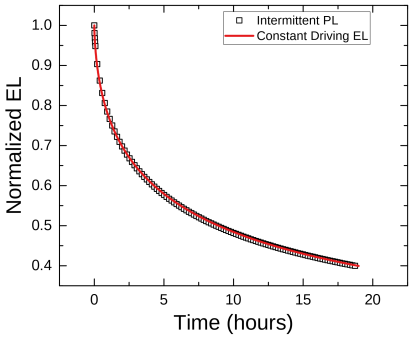
\includegraphics[width=0.48\textwidth]{integratedLifetime/lifetime_vs_drive}
\caption{Lifetime obtained under a constant driving current is shown in red solid line.  Lifetime under the same conditions but with PL measurement breaks is shown in open squares.  Strong agreement is observed.}
\label{fig:lifetime_vs_drive}
\end{wrapfigure}

where $L_{PL}$ is the experimentally measured luminance, $I$ is the pump intensity, and $\alpha$ is the film absorption.
The pump intensity, $I$, can be measured and is observed to remain constant within error during the degradation.
The absorption, $\alpha$, has also been measured before and after degradation, and is found to be constant within error.
However, the sensitivity of the absorption measurement may not reflect the sensitivity of the \pl measurement.
An alternative method to verifying the \pl measurement is presented in Section \ref{sec:lifetime_pl_transients}.


In traditional lifetime measurements, constant current density excitation is used.  
In order to measure \pl as well, the current is paused every 10 minutes long enough to stabilize the laser and take a measurement, before the current is resumed.
This takes on the order of 20 seconds, and is shown in Figure \ref{fig:schematic}b.
To make these measurements comparable with traditional lifetimes, time is reported as the elapsed time under electrical current, with the laser breaks subtracted.
This method has been shown to accurately match the traditional lifetime measurements, without additional degradation due to the PL measurement or relaxation from the breaks in current, as shown in Figure \ref{fig:lifetime_vs_drive}.

The accuracy of this measurement technique relies heavily on several testing considerations and assumptions.
Important considerations of testing conditions and sources of error are discussed in the following sections.

\subsection{Light Selection}

Light sources for optical pumping are required to be powerful enough to pump the emitter sufficiently for measurement, stable enough to maintain output power for lifetimes over 100 hours, and long lived.
Ideal candidates are lasers and high power lamps, though lamps often have a long warmup time, which is not ideal for the short on time needed for this experiment.
Lamps do have the advantage that they can pump all of the device active area, getting a better sample of the behavior, though lasers can be expanded for the same effect.

\begin{wrapfigure}{r}{.5\textwidth}
\centering
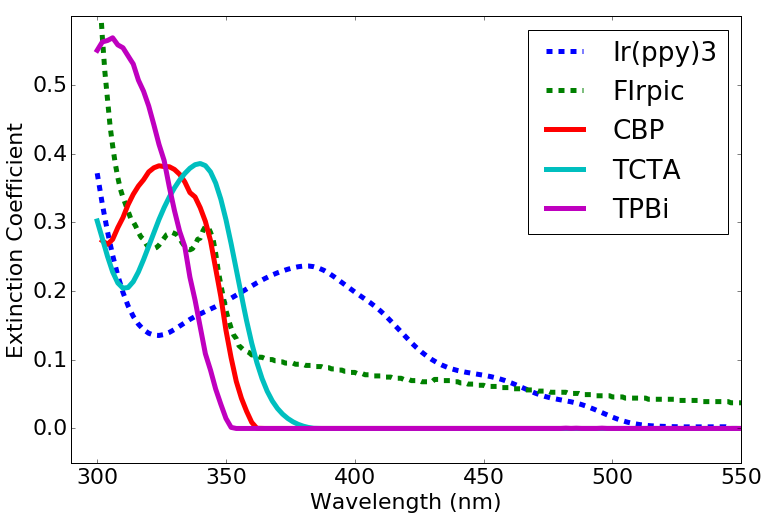
\includegraphics[width=0.48\textwidth]{integratedLifetime/optical_k}
\caption{Extinction coefficients shown for the green emitter \irppy and blue emitter Fir(pic) as well as a few host materials.}
\label{fig:optical_k}
\end{wrapfigure}

During the optical pumping, it is important to only pump the emissive layer, and for the most direct measurement of \pl, only the emitter molecule.
To accomplish this, careful selection of wavelength must occur.  
Figure \ref{fig:optical_k} shows the optical extinction coefficient for several materials.  
Ideally, the pump wavelength should be selected so that the emitter molecule has significant absorption, but the host does not.  
This is relatively easy for the green emitter, \irppy where a wide range of pumps would work between 375 and 500 nm.
However, This becomes extremely difficult for blue emitters such as Fir(pic), where hosts are more resonant with the emitter.  
In this case, the host may have to be pumped and exciton transfer from the host to the guest will be included in the measurement.
Even with this, the transport layers would have to have higher triplet energies than the emitter.

Due to these limitations, lasers are ideal light sources for green emitters, since they are easily manipulated optically to pump multiple devices.
Here, the limitations of available laser wavelengths are less important due to the wide pumping window.
However, for blue emitters, a lamp may be a more viable option as it would allow filtering or monochromation to be more selective of wavelength.



\subsection{Absorption - Recombination Overlap}\label{sec:abs_rz_overlap}

\begin{wrapfigure}{r}{.5\textwidth}
\centering
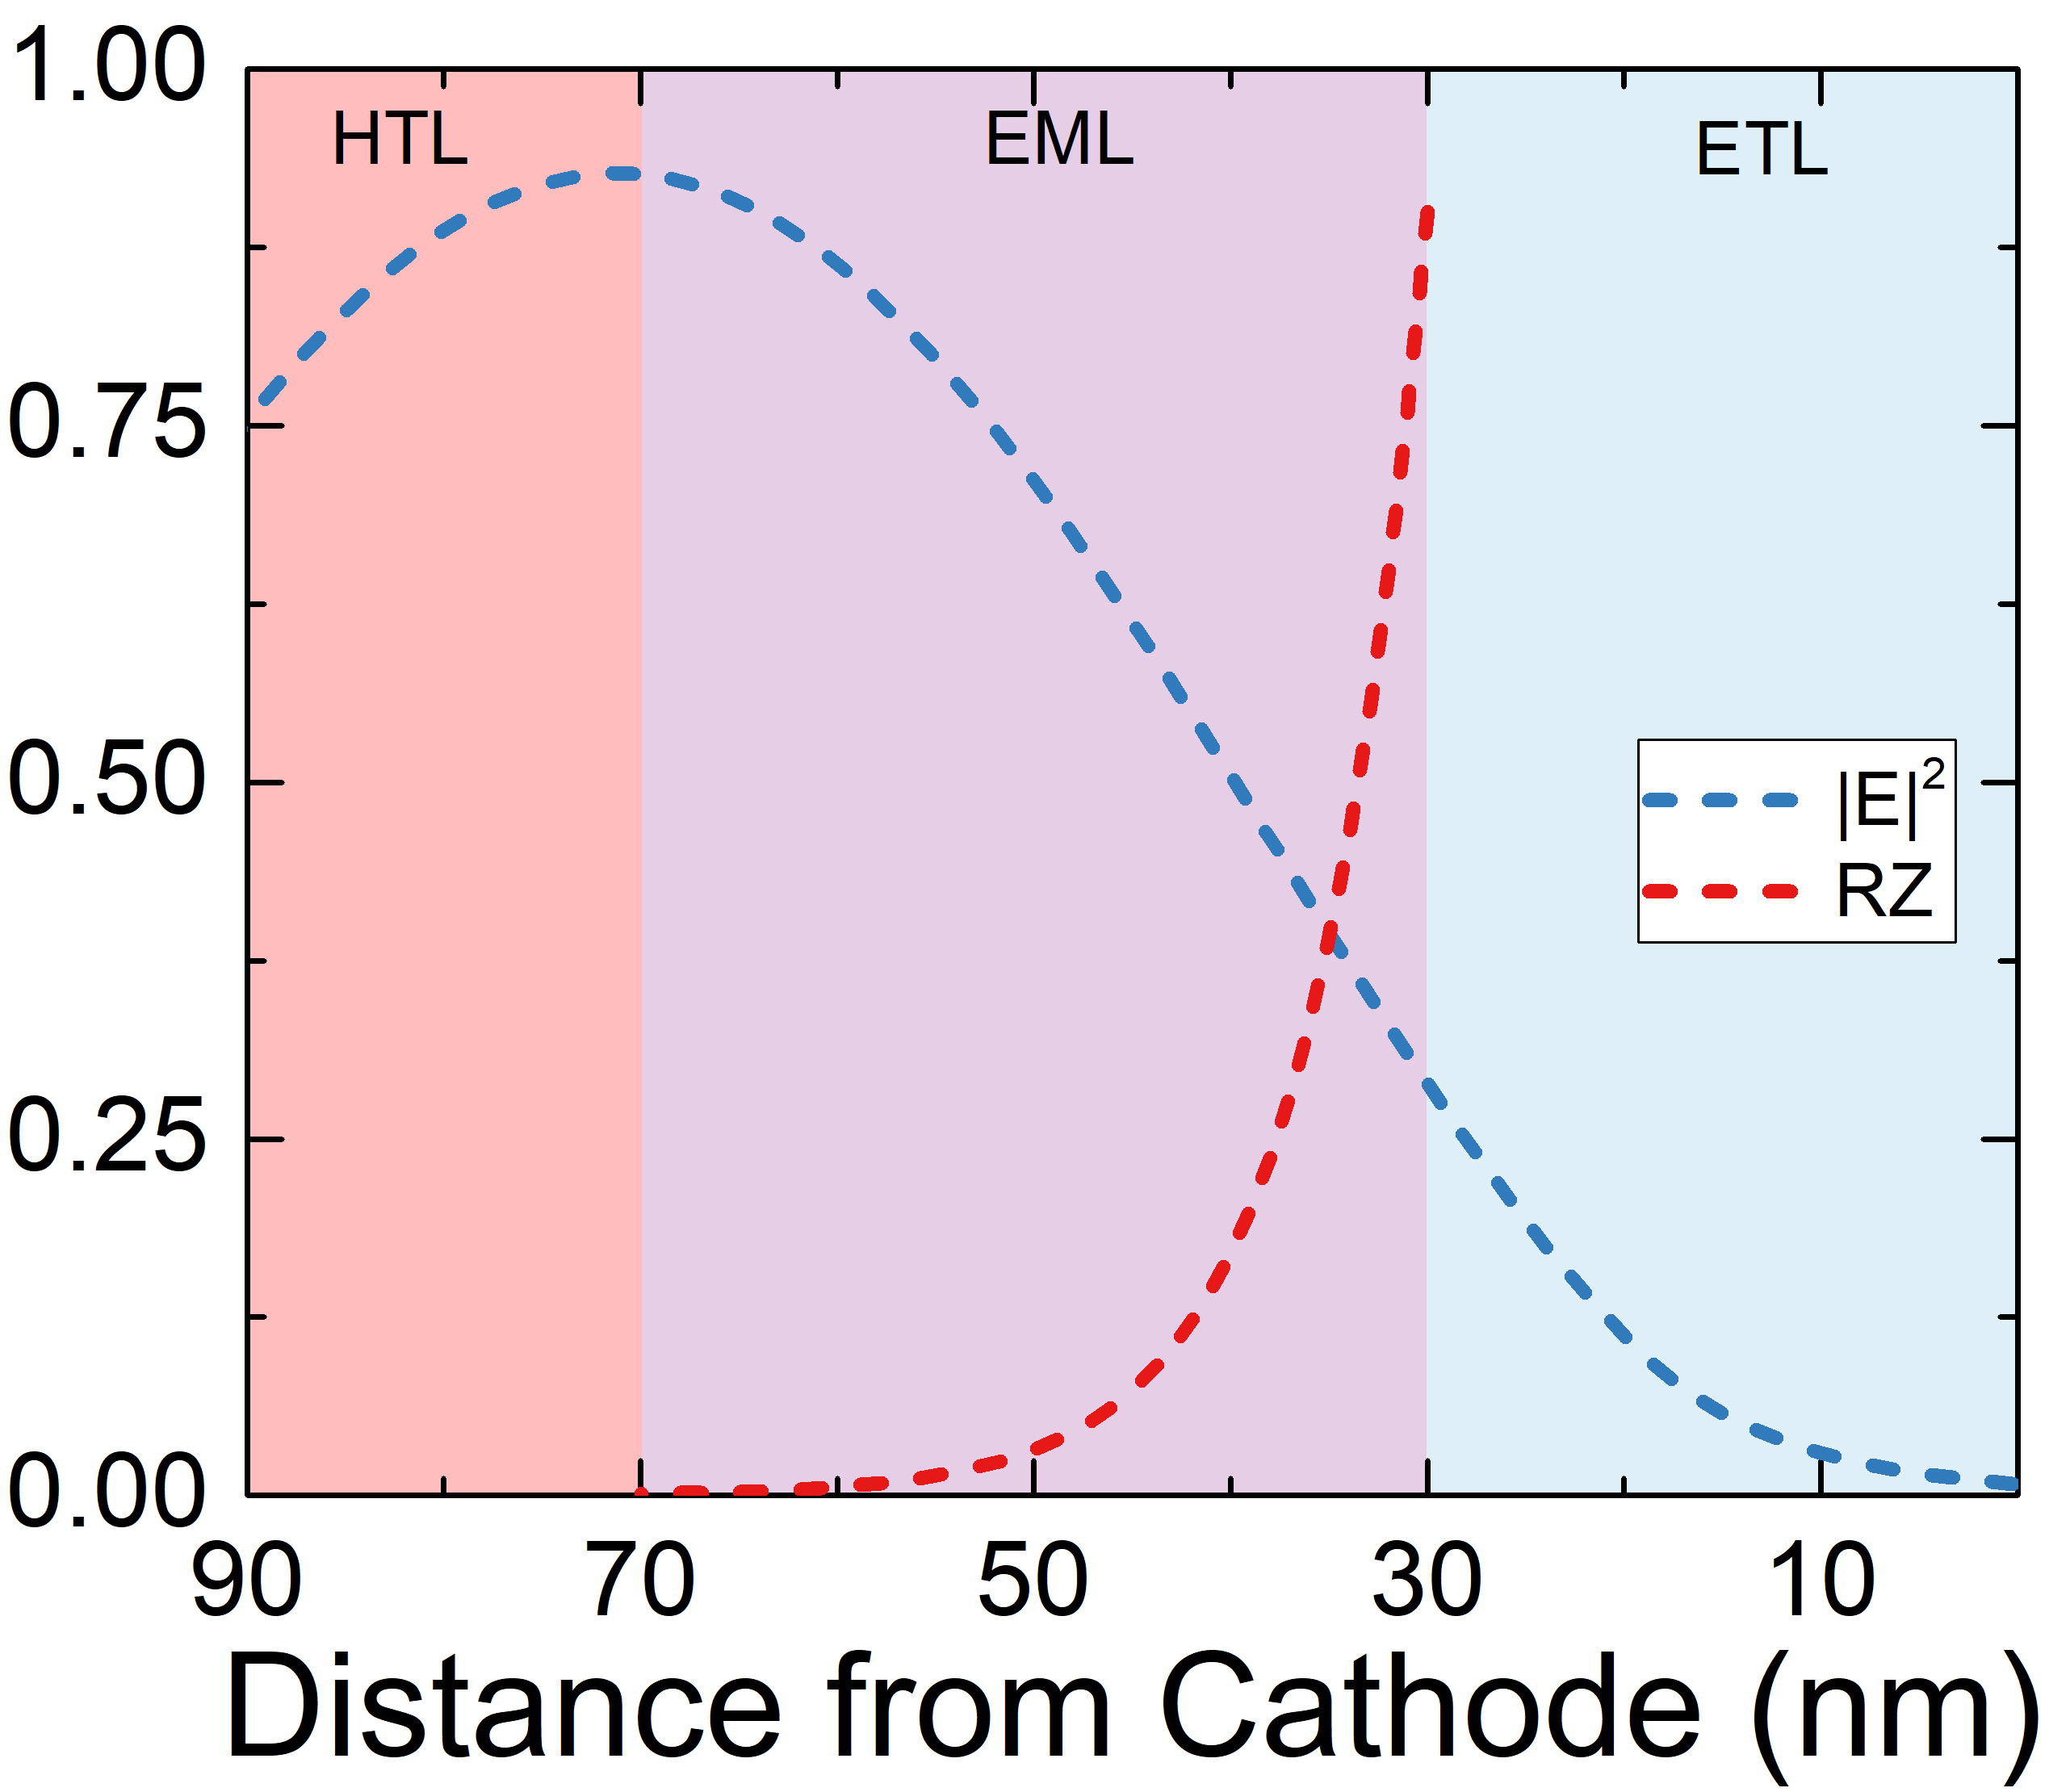
\includegraphics[width=0.48\textwidth]{integratedLifetime/rz_field_overlap}
\caption{Exciton recombination zone (RZ) and pump intensity $|E|^2$ for a hypothetical thick EML device are shown.}
\label{fig:rz_abs_overlap}
\end{wrapfigure}


For the measurement of \pl to accurately reflect the useful degradation of the emissive layer, it is important for the optical pump absorption to agree with the recombination zone within the device.  
To illustrate this, Figure \ref{fig:rz_abs_overlap} shows a device where there is disagreement between the absorption and the recombination zone.  
Assuming an exciton driven process, defect formation and degradation will focus around the recombination zone.
However, optical measurements will probe in the absorption region, which is less degraded than the electrically driven luminance is reflecting.
This leads to a systematic underestimate of the actual \pl degradation within the device.

To quantify this error for a particular device, a degradation and defect generation model must be employed in order to quantify the degradation profile within the device.  
Additionally, the absorption profile and recombination zone must be known (or estimated).
The absorption profile can be calculated using a transfer matrix formalism.\supercite{Pettersson1999}
The code used to calculate this is provided in Appendix \ref{sec:outCoupling_code}.
The recombination zone can be measured using sensitizer molecules using the method outlined in Chapter \ref{sec:rz_measurement}.
An excellent example of executing this analysis demonstrated by \textcite{Bangsund2018}


\subsection{Contact Degradation}

\begin{wrapfigure}{r}{.5\textwidth}
\centering
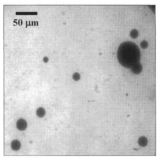
\includegraphics[width=0.48\textwidth]{integratedLifetime/dark_spot}
\caption{Dark spot formation on a device after exposure to a 405 nm laser.}
\label{fig:dark_spot}
\end{wrapfigure}

Exposure to UV light has been shown to enhance photodegradation of the organic/LiF/Al interface within devices.\supercite{Wang2011a,Wang2010a}
This has been shown to be due to the dissociation and diffusion of positive ions from this interface, likely due to LiF.
This becomes problematic in this measurement due to the \pl measurement, as illustrated in Figure \ref{fig:dark_spot}.
Here, the optical pump as formed a dark spot on the active area of the device and accelerated degradation.

To minimize this behavior, the laser intensity incident on the device must be kept low.
We have found through trial and error that incident powers below 10 mW/cm$^2$ for a 405 nm laser do not exhibit this dark spot formation.
Devices can be inspected after lifetime testing to ensure that no degradation occurred.  
We have also observed that for longer wavelengths, the damage power threshold increases and higher power can be used.

\subsection{Quenching Changes During Degradation}\label{sec:eta_tau}

\begin{wrapfigure}[13]{r}{.5\textwidth}
\centering
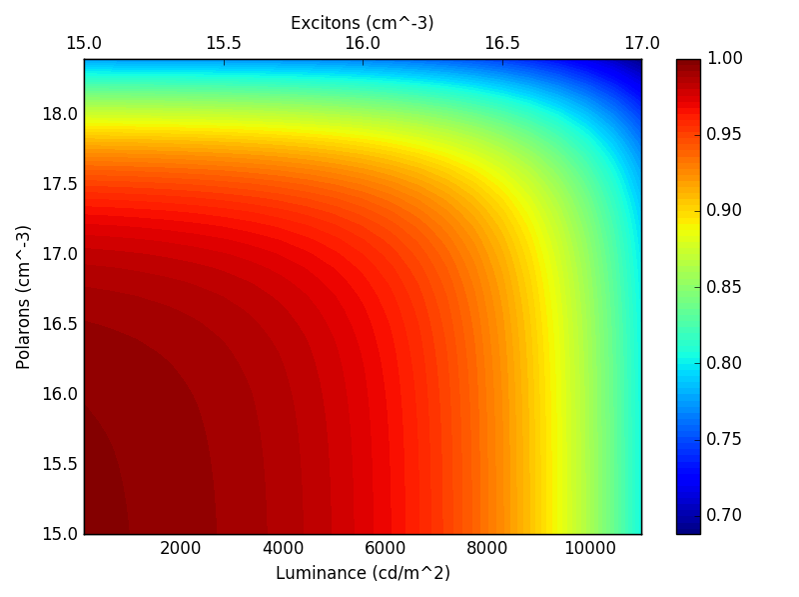
\includegraphics[width=0.48\textwidth]{integratedLifetime/quenching_correction}
\caption{Multiplicative correction factor for exciton formation efficiency due to changes in quenching during lifetime.  Shown as a function of polaron and exciton density as well as luminance, assuming a 10 nm emissive layer.}
\label{fig:quenching_correction}
\end{wrapfigure}


Equation \ref{eqn:eqe_quenching} introduces a quenching term, $\eta_\tau$, into \eqe.  
This term captures bimolecular quenching losses which occur at high current and exciton densities.
During lifetime measurements, the exciton density decreases as the efficiency reduces, which will change $\eta_\tau$.
To quantify this, the model presented in Chapter \ref{sec:unified} can be used.
Using this dynamics formalism, we can define $\eta_\tau$ as

\begin{equation}
\eta_\tau=\frac{1/\tau}{1/\tau+\frac{1}{2}\ktt n_{ex} +\ktp n_{pol}}.
\label{eqn:eta_tau}
\end{equation}

To find $\eta_\tau$ at the end of degradation, the change in $n_{ex}$, $n_{pol}$, and $\tau$ must be known.  
The change in $\tau$ is known from \pl. as discussed in Section \ref{sec:lifetime_pl_transients}.
The exciton population, $n_{ex}$, is known from luminance as discussed in Chapter \ref{sec:unified} and the temporal dependence follows the luminance loss assuming the radiative rate remains constant (which we assume).
The polaron population likely increases to account for the decrease in our exciton density, but is difficult to quantify.
Therefore, for this argument, we will assume it remains constant, though it will likely counteract some of the error that this method will estimate.
With the temporal dependence of these quantities known, the time dependence of Equation \ref{eqn:eta_tau} can be written as


\begin{equation}
\frac{\eta_\tau(t)}{\eta_\tau^0}=\frac{1/\tau}{1/\tau+\frac{1}{2}\ktt n_{ex} +\ktp n_{pol}}  \frac{1/(R_{PL}(t)\tau)+\frac{1}{2}\ktt (R_{EL}n_{ex}) +\ktp n_{pol}}{1/(R_{PL}(t)\tau)}
\label{eqn:eta_tau_deg}
\end{equation}

where $R_X$ is the degradation ratio of that term.  
Since degradation decoupling results are presented assuming $\eta_\tau(t)=C$, the presented out-coupling results can be corrected using $\eta_\tau^0/\eta_\tau(t)$ as a multiplicative correction factor, presented in Figure \ref{fig:quenching_correction}.
In this figure, minimal correction is needed for low exciton and polaron populations.  
This only becomes important in regimes where bimolecular quenching are strong.
Again, it is important to note that if changes in the polaron population are accounted for, this correction factor would be further reduced.

\subsection{Verification with Exciton Lifetime}\label{sec:lifetime_pl_transients}
\begin{wrapfigure}{r}{.5\textwidth}
\centering
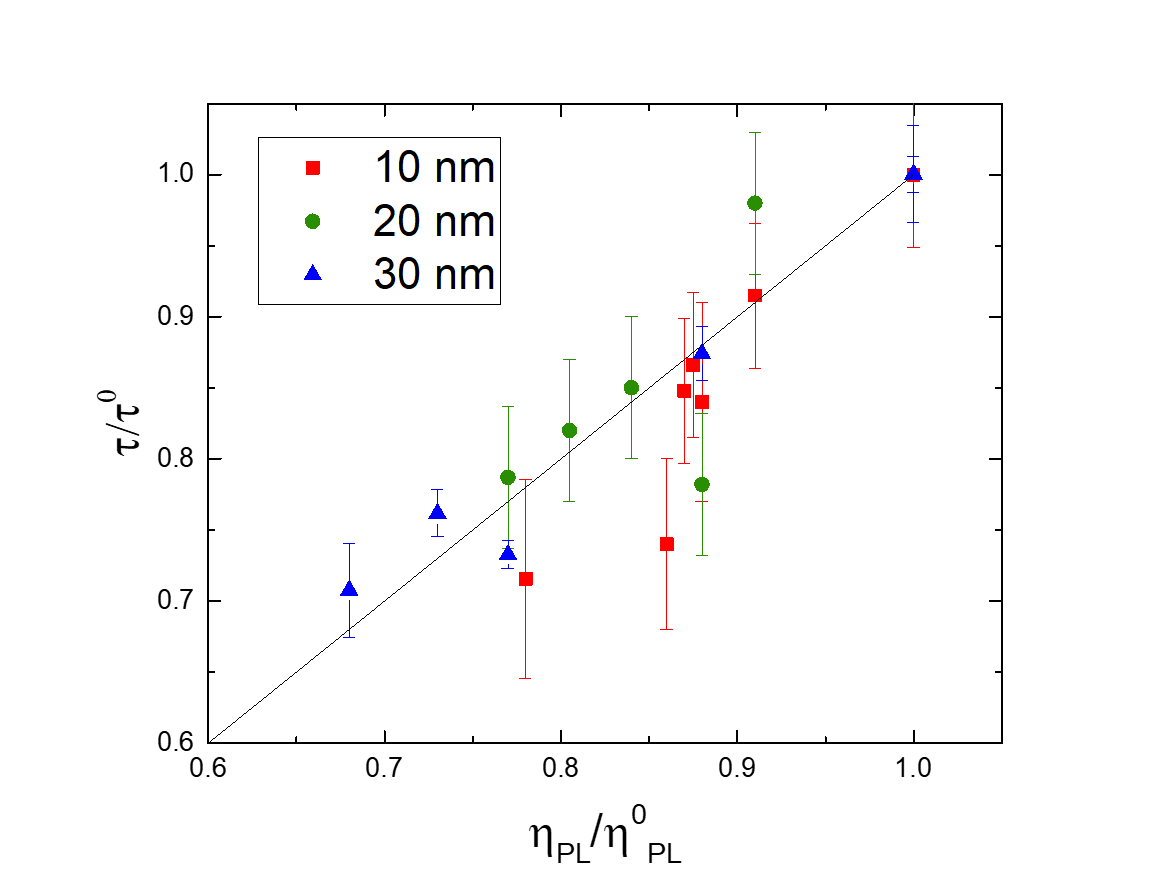
\includegraphics[width=0.48\textwidth]{integratedLifetime/transient_lifetimes}
\caption{Exciton lifetime ratio extracted from transient PL measurements on degraded and undegraded devices as a function of PL degradation for several emissive layer thickness.}
\label{fig:transient_lifetimes}
\end{wrapfigure}


Alternative to the method for establishing the accuracy of the \pl degradation presented in Equation \ref{eqn:pl_decay}, the exciton lifetime can be used.
From photophysics, we have

\begin{align}
\pl=\frac{k_r}{k_r+k_{nr}} && \tau=\frac{1}{k_r+k_{nr}}
\label{eqn:tau_pleff}
\end{align}

where $k_r$ and $k_{nr}$ are the radiative and non-radiative decay rates, respectively.
From these equations, it is apparent that if $k_r$ remains constant during the degradation, 

     \[\frac{\tau(t)}{\tau^0}=\frac{\pl(t)}{\pl^0}\]


Therefore, if the exciton lifetime, $\tau$ is measured as a function of decay, it should have a 1-to-1 correlation with the observed PL loss if an accurate measure of \pl is being conducted.  
To do this, $\tau$ is measured from the transient photoluminescence decay at low pump intensity so that minimal triplet-triplet annihilation is observed. 
This is done on a 337 nm pulsed nitrogen laser, recorded with a fast photodiode connected to an oscilloscope.
This have been done for a variety of device architectures, an example of the results being shown in Figure \ref{fig:transient_lifetimes} for the devices discussed in Chapter \ref{sec:cbp_host}.
Here we see that we are accurately measuring \pl for this device since a strong correlation is observed.  
The large amount of scatter observed in the 10 nm EML results are believed to be due to the thin EML and small amount of material, producing low signal.

It is important to note for this confirmation of \pl, that this only demonstrates that no absorption or pump intensity deviations are causing error in our measurement.
Since the transient photoluminescence and photoluminescence degradation are both pumped optically, both are subject to the recombination zone and absorption mismatch problem discussed in Section \ref{sec:abs_rz_overlap}.



\section{Experimental Implementation}
\subsection{Hardware Setup}

\begin{figure}[ht]
    \begin{minipage}{\linewidth}
    \centering
    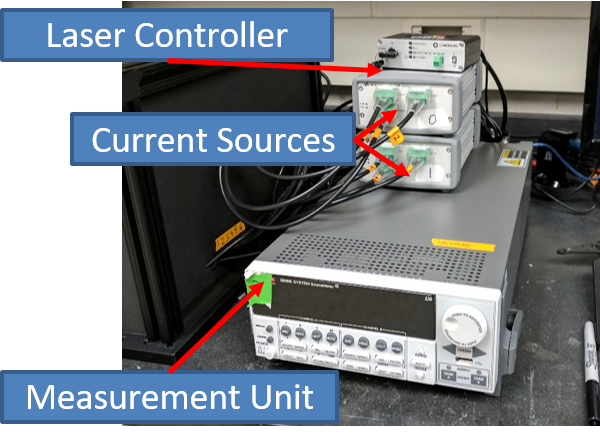
\includegraphics[height=2in]{integratedLifetime/source_measure}
    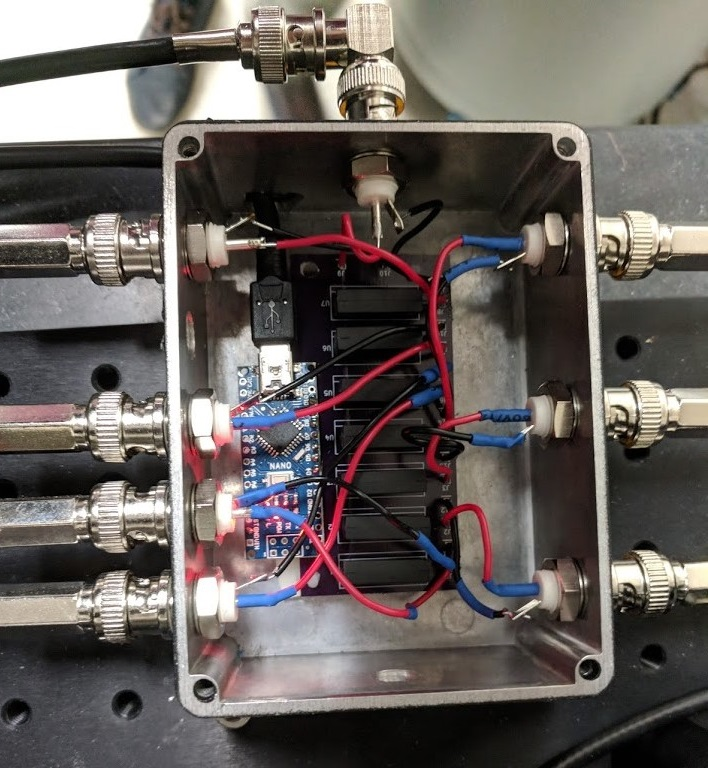
\includegraphics[height=2in]{integratedLifetime/arduino}
    \caption{Source-Measure hardware and laser controller}
    \label{fig:source_measure}
    \end{minipage}
\end{figure}

Hardware for this setup requires control of current sources, voltage measurement, light source, as well as light measurements. 
Currently, there are four operational testing setups, termed ``boxes'', with varying hardware configurations.
Several boxes are multiplexed to allow multiple measurements from the multiple compartments.
Source units for providing current and voltage measurements have used either the Keithley 26xx or Keysight u2722a source meters.  
The Keithley 26xx units are a two channel, low noise, high precision unit.
The Keysight u2722a provides three channels with higher noise and lower precision at a lower price point per channel.
Light sources for all boxes are conducted using Coherent OBIS lasers, with wavelengths of either 405 nm or 473 nm.
Light measurements are conducted using the Keithley 26xx for all boxes, connected to a Hamamatsu S2281 photodiode.
Figure \ref{fig:source_measure}a shows the electronic hardware
\begin{wrapfigure}{r}{.5\textwidth}
\centering
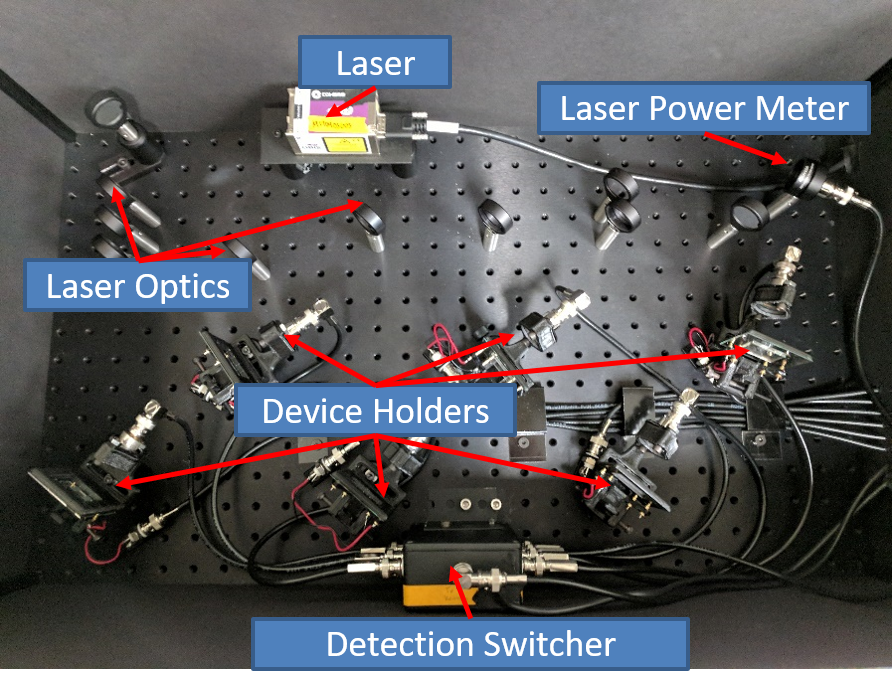
\includegraphics[width=0.48\textwidth]{integratedLifetime/hardware}
\caption{Device contacting, measurement, and optical hardware.  Version 3 of the hardware is shown.  Controlling hardware is shown in Fig. \ref{fig:source_measure}}
\label{fig:hardware}
\end{wrapfigure}
 setup for a box utilizing Keysights for source units and a Keithley for measurement.
To reduce measurement units, the photodiodes in each compartment can be switched between using an Arduino relay system shown in Figure \ref{fig:source_measure}b.
All of these pieces of hardware are compatible with the National Instrument VISA command library for control.


Each device is held by a custom 3D printed vertical mount.  
The photodiode is wired into this mount with enough space for the laser to avoid the diode.
A long pass filter is provided to minimize stray laser signal.
The laser is optically split into six paths using beam splitters and neutral density filters are used where necessary to normalize laser power on each device.


\subsection{Software Development}

\begin{figure}[ht]
    \centering
    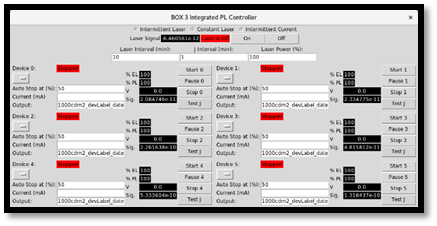
\includegraphics[width=0.8\textwidth]{integratedLifetime/software_controller}
\caption{6 channel software controller.  Selection of test type, laser control for alignment, and global settings are accessible on the top of the interface.  Individual channel settings are grouped on the bottom.}
\label{fig:software_controller}
\end{figure}

Software to control this measurements is implemented by myself in Python and outlined in Appendix \ref{sec:lifetime_code}.
The code is able to control the hardware to run constant current, intermittent laser integrated PL measurements, optical degradation, as well as optical degradation with current break degradations.
The frequency of laser breaks and laser power can be controlled on a whole box level.  
Laser emission can be turned on for alignment.
The software is able to be configured to the number of channels available depending on the hardware.
Each channel can be individually controlled for current, stop, and labeling.  

\begin{figure}[ht]
    \centering
    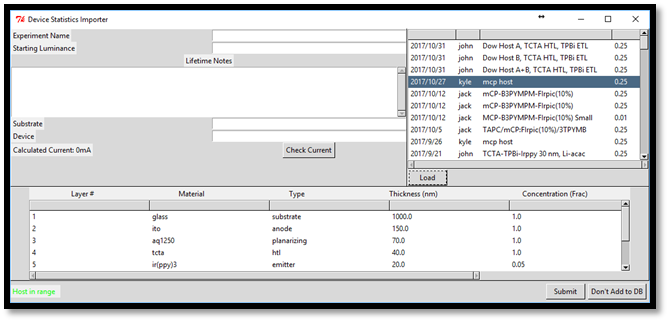
\includegraphics[width=0.8\textwidth]{integratedLifetime/lifetime_db_import}
\caption{Test information for database import interface.  The top left panel collects information about the specific device and lifetime.  The right panel connects the device to a particular growth and architecture.  The bottom panel confirms the architecture.}
\label{fig:lifetime_db_import}
\end{figure}

To organize collected data, a database for all lab data has been developed and is discussed in Chapter \ref{sec:data}.
Lifetimes integrate with this system when lifetimes are started, using the interface shown in Figure \ref{fig:lifetime_db_import}.
Here, a lifetime test is connected to a particular growth, as well as the individual substrate and device pixel. 
Information about the lifetime is also connected.  
The lifetime operating current can be determined for a desired luminance by utilizing the current-voltage-luminance curve for the exact device within this interface.  
Additional notes and information are also able to be stored.

\section{Conclusion}
This chapter has outlined a system for decoupling degradation during operational lifetimes.
Extensive care has been taken to outline the assumptions and assess error within the extracted parameters.  
Many of these assumptions need to be assessed for any device system to be tested to ensure accuracy.  
Applying this method to lifetime decoupling in device systems is the subject of Chapter \ref{sec:decoupling_applications}.



\ifcsdef{mainfile}{}{\printbibliography}
\end{document}
